\chapter{Controlled Spatial Transformation With Deterministic Mapping Function}
\section{Introduction}


 In Chapter 2, we elaborated on the details of the patient-adaptive ECG classification framework. An important part of this methodology is to design a \textit{personalized classifier} with a \textit{deviation analysis module}. The performance of the \textit{deviation analysis module} depends on the geometry of different classes of data samples in the feature space. In Chapter 3, we proposed a novel spatial transformation method based on MOPSO to  achieve a desired symmetry in the transformed feature space to boost the performance of the deviation analysis module. This methodology enables us to further process the normal samples and identify fuzzy states between the normal and abnormal states. However, the proposed method uses an iterative optimization which may have high computational complexity. In this chapter, we introduce another deterministic spatial transformation method to model the fuzzy state of samples with a more tractable and analytical solution. %These two methods share a common concept of modeling the intermediate states from annotated normal to abnormal state. 

 
While the aforementioned method in Chapter 3 yields the desired capacity of predicting upcoming abnormalities, the interpretation of the mechanisms of the system is not straightforward and easily tractable, thus it is not easily generalizable to a broader range of applications in the biomedical signal processing. The main objective of this chapter is to develop a deterministic transformation with a stronger prediction power based on a controlled spatial topology studied in Chapter 3. In this method, we further optimize the topology and spatial geometry of the clusters in the feature space by reducing the within-cluster variance after the spatial transformation. As shown in Fig. \ref{fig:topo2}, through this improvement, the performance of the personalized classifier in terms of prediction accuracy can be further enhanced with the proposed method.
 
%Having analyzed the symmetric encircled topology in the previous chapter, we proposed a novel spatial transformation based predictive modeling system to assist cardiologist take advanced therapeutic Interventions. In this method, we further optimize the topology and spatial geometry of clusters in the feature space by reducing the within cluster variance after spatial transformation. As shown in \ref{fig:topo2}, through this improvement, the predicting accuracy of personal classifier can be further improved.
\begin{figure}[t]
\centering
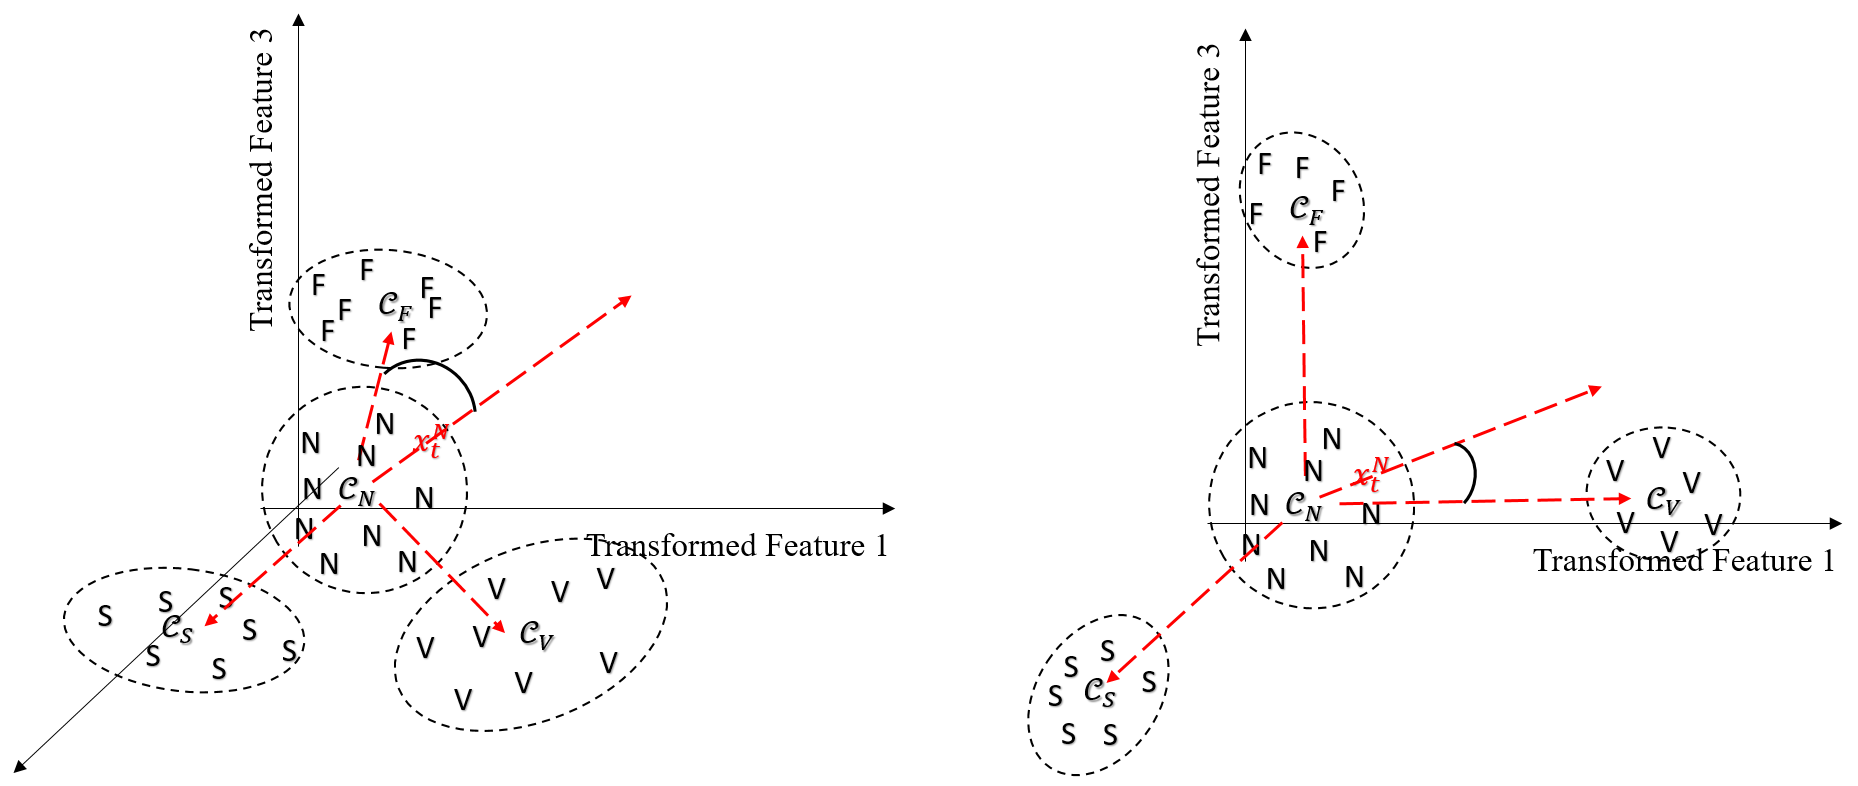
\includegraphics[scale=.42]{Fig/topo2.png}
\caption{Left: illustration of the clustering topology in the \textcolor{blue}{original} feature space; % transformed with a simple mapping function;  
Right: illustration of the clustering topology in the feature space transformed with an optimized mapping function. \textcolor{red}{Razi: it is not clear what you mean here by simple, is it unoptimized, why not just saying the original space before transmission !}}
\label{fig:topo2}
\end{figure}

\section{Hyper-Spherical Coordinates}

In the previous chapter, the spatial transformation module is implemented with a polynomial kernel function and a heuristic optimization method. The system performance has been proven to be promising. In addition to the general drawbacks of heuristic method, it is not straightforward to select an appropriate base kernel as the core of spatial mapping function due to the high variety of kernel functions. % and the limitation of dimensionality.

In order to address this issue, a novel deterministic spatial mapping function is proposed in this chapter based on \textit{hyper-spherical} coordinates [REF: XXX (it is ok to repeat references, ans is ok to have web pages as REFs)]. Since hyper-spherical coordinates consist of angles and radii, these parameters in both original feature space and the desired target space are used to determine the mapping function.


The hyper-spherical coordinate system (n-dimensional spherical coordinate system) and its mapping to the \textit{Cartesian} coordinate system are first introduced in \cite{nsphere}. If $\mathbf{x}$ is a sample vector in 
a $n$-dimensional feature space, with its Cartesian coordinates $(\xi_1,~\xi_2~... \xi_n)$, then its corresponding hyper-spherical coordinates can be obtained through Eq.\ref{eq:cart2sph}, which is originally derived through its reverse mapping (Eq.\ref{eq:sph2cart}) using equation: $\sin(\arccos(x)) = \sqrt{1-x^2}$.



\begin{align}
\label{eq:cart2sph}
\nonumber
r      &= \sqrt{{\xi_n}^2 + {\xi_{n-1}}^2 + \cdots + {\xi_2}^2 + {\xi_1}^2} \\
\nonumber
\theta_1 &= \arccos \frac{\xi_{1}}{\sqrt{{\xi_n}^2+{\xi_{n-1}}^2+\cdots+{\xi_1}^2}} \\
\nonumber
 \theta_2 &= \arccos \frac{\xi_{2}}{\sqrt{{\xi_n}^2+{\xi_{n-1}}^2+\cdots+{\xi_2}^2}} \\
\nonumber
        &\vdots\\
\nonumber
 \theta_{n-2} &=\arccos \frac{\xi_{n-2}}{\sqrt{{\xi_n}^2+{\xi_{n-1}}^2+{\xi_{n-2}}^2}} \\
 \theta_{n-1} &= 
 \begin{cases}
     \arccos \frac{\xi_{n-1}}{\sqrt{{\xi_n}^2+{\xi_{n-1}}^2}} & \xi_n\geq 0 \\
     - \arccos \frac{\xi_{n-1}}{\sqrt{{\xi_n}^2+{\xi_{n-1}}^2}} & \xi_n < 0
 \end{cases} 
\end{align}


\begin{align}
\label{eq:sph2cart}
\nonumber
\xi_1 &= r \cos(\theta_1) \\
%\xi_j &= r \cos(\theta_j)\prod_{k=1}^{j-1}\sin(\theta_k)\\
\nonumber
\xi_2 &= r \sin(\theta_1) \cos(\theta_2) \\
\nonumber
\xi_3 &= r \sin(\theta_1) \sin(\theta_2) \cos(\theta_3) \\
\nonumber
    &\vdots\\
\nonumber
\xi_{n-1} &= r \sin(\theta_1) \cdots \sin(\theta_{n-2}) \cos(\theta_{n-1}) \\
\xi_n &= r \sin(\theta_1) \cdots \sin(\theta_{n-2}) \sin(\theta_{n-1}).
\end{align}


where $0\leq \theta_j\leq\pi,~j=1,\dots ,n-2$; $0\leq \theta_{n-1}\leq 2 \pi$; $0\leq r<\infty$
 
 
\section{Orthogonalization}

To simplify the algorithm, in this chapter, the topology of clusters in feature space is approximated by relative location of cluster centroids: $\mathbf{c}_N^k, \mathbf{c}_{\mathcal{V}}, \mathbf{c}_{\mathcal{S}}, \mathbf{c}_{\mathcal{F}}$. Furthermore, as we assume that the samples with fuzzy state deviate from normality to abnormality, the spatial topology stays unchanged if normal centroid is simply translated to the origin in Cartesian coordinate. The cluster topology in original feature space can be equivalently represented by the following matrix with three row vectors:

\begin{align}
\mathcal{C} = 
\begin{bmatrix}
\mathbf{c}_{\mathcal{V}} - \mathbf{c}_N^k \\
\mathbf{c}_{\mathcal{S}} - \mathbf{c}_N^k \\
\mathbf{c}_{\mathcal{F}} - \mathbf{c}_N^k
\end{bmatrix} = 
\begin{bmatrix}
\mathbf{V}_{\mathcal{VN}} \\
\mathbf{V}_{\mathcal{SN}} \\
\mathbf{V}_{\mathcal{FN}}
\end{bmatrix}
\end{align}

As shown in Fig. \ref{fig:topo2}, in order to improve personalized classifier and avoid ambiguity, a topology with maximum separation between three vectors in $\mathcal{C}$ is preferred. To lower computational complexity in high dimension, the algorithm aims at transforming vectors in $\mathcal{C}$ to orthogonal vectors with deterministic functions. Therefore, the method proposed in \cite{Gram-schmidth2} based on the well known orthogonalization method \textit{Gram-Schmidt} in \cite{Gram-schmidth1} is deployed. Hence, in the first step of the function, the three row vectors in $\mathcal{C}$ representing the centroids is fed to the orthogonalization process as follows:
\begin{align}
\mathcal{C}^{\perp}= \text{Gram-Schmidt}(\mathcal{C})
=
\begin{bmatrix}
\mathbf{V}_{\mathcal{VN}}^{\perp} \\
\mathbf{V}_{\mathcal{SN}}^{\perp} \\
\mathbf{V}_{\mathcal{FN}}^{\perp}
\end{bmatrix}
\end{align}

where $\mathcal{C}^{\perp}$ is the matrix of orthogonalized vectors in Cartesian coordinates. The hyper-spherical coordinates $\mathcal{C}^{\perp}_{*}$ of these orthogonalized vectors are calculated subsequently using Eq.\ref{eq:cart2sph}. After this step, the orthogonalized vectors in hyper-spherical coordinates are obtained as formulated in Eq. \ref{eq:c_ortho}. The $j$th angular dimensions are noted as  $\theta_{j}^{\perp}$ and the radius dimension is noted as $r^{\perp}$%, which reveals the angular change from original vectors to the ideal orthogonal vectors, are calculated subsequently using Eq.\ref{eq:cart2sph}.

\begin{align}
\label{eq:c_ortho}
\mathcal{C}^{\perp}_{*} =
\begin{bmatrix}
    r_{\mathcal{VN}}^{\perp} & \theta_{1_{\mathcal{VN}}}^{\perp} & \dots  & \theta_{{n-1}_{\mathcal{VN}}}^{\perp} \\
    r_{\mathcal{SN}}^{\perp} & \theta_{1_{\mathcal{SN}}}^{\perp} & \dots  & \theta_{{n-1}_{\mathcal{SN}}}^{\perp} \\
%    \vdots & \vdots & \ddots & \vdots \\
	r_{\mathcal{FN}}^{\perp} & \theta{1_{\mathcal{FN}}}^{\perp} & \dots  & \theta_{{n-1}_{\mathcal{FN}}}^{\perp} \\
\end{bmatrix}
\end{align}


\section{Spatial Mapping Function}
After obtaining the original hyper-spherical coordinates of $[\mathbf{V}_{\mathcal{VN}},~\mathbf{V}_{\mathcal{SN}},~\mathbf{V}_{\mathcal{FN}}]^T$ and orthogonalized hyper-spherical coordinates $[\mathbf{V}_{\mathcal{VN}}^{\perp},~\mathbf{V}_{\mathcal{SN}}^{\perp},~\mathbf{V}_{\mathcal{FN}}^{\perp}]^T$, the goal is to design a mapping function $\mathbf{F}: \mathbf{R}^n \to \mathbf{R}^n$ from the original coordinates to the orthogonal ones which represent the ideal cluster topology.

In Gram-Schmidt algorithm, the very first vector of the input vector array serves as a reference vector and remains unchanged in the orthogonalized vector array. As a result, $\mathbf{V}_{\mathcal{VN}} = \mathbf{V}_{\mathcal{VN}}^{\perp}$ and $\mathbf{F}$ can be equivalently defined by the following equations:

\begin{align}
\label{eq:constraints}
\begin{aligned}
%\mathbf{F}(0) &= 0 &~\\
\mathbf{F}(\mathbf{V}_{\mathcal{SN}} - \mathbf{V}_{\mathcal{VN}}) &= \mathbf{V}_{\mathcal{SN}}^{\perp} - \mathbf{V}_{\mathcal{VN}}^{\perp} &= \mathbf{V}_{\mathcal{SN}}^{\perp} - \mathbf{V}_{\mathcal{VN}}\\
\mathbf{F}(\mathbf{V}_{\mathcal{FN}} - \mathbf{V}_{\mathcal{VN}}) &= \mathbf{V}_{\mathcal{FN}}^{\perp} - \mathbf{V}_{\mathcal{VN}}^{\perp} &= \mathbf{V}_{\mathcal{FN}}^{\perp} - \mathbf{V}_{\mathcal{VN}}
\end{aligned}
\end{align}

Furthermore, since orthogonality is independent to radius dimension $r$, we only need to design $\mathbf{F}$ for $n-1$ dimensions, which includes all angular dimensions ($\theta_1,\dots,\theta_{n-1}$), and coordinate $r$ remains unchanged before and after mapping. Consequently, the determination of $\mathbf{F}$ can be decomposed to the determination of $n-1$ functions: $f_i: \mathbf{R}\to \mathbf{R},~i=1\dots n-1$ with constraints in Eq.\ref{eq:constraints} and boundary constraints of angular dimensions. %In order to standardize $f_i$ for all angular dimensions, $\theta_i, ~i=1\dots n-2$ are proportionally scaled to the range between $(0,2\pi)$.
We note $\mathbf{V}_{\mathcal{SN}} - \mathbf{V}_{\mathcal{VN}} = \Delta_{\mathcal{SV}}$ and the $i$th angular dimension of $\Delta_{\mathcal{SV}}$ as $\delta_{i_{{\mathcal{SV}}}}$. Same notation is applied on $\mathbf{V}_{\mathcal{FN}} - \mathbf{V}_{\mathcal{VN}}$. %Hence for each angular dimension $i, i = 1,\dots, n-2$, $\delta_{i_{{\mathcal{SV}}}}$ and $\delta_{i_{{\mathcal{FV}}}}$ are both within the range of $(-\pi,\pi)$
Hence for each angular dimension $i$, $f_i$ is determined by ($\delta_{i_{{\mathcal{SV}}}}$,$\delta^{\perp}_{i_{{\mathcal{SV}}}}$) and ($\delta_{i_{{\mathcal{FV}}}}$,$\delta^{\perp}_{i_{{\mathcal{FV}}}}$), together with two boundary constraints of angular dimensions.
%if $f_i$ is to be depicted with a curve in 2-D plane, this curve will 4 points: (0,0), ($\delta_{i_{{\mathcal{SV}}}}$,$\delta^{\perp}_{i_{{\mathcal{SV}}}}$), ($\delta_{i_{{\mathcal{FV}}}}$,$\delta^{\perp}_{i_{{\mathcal{FV}}}}$), ($\pi$, $\pi$)

In order to maintain the simplicity and linearity of the mapping function, $f_i$ needs to be continuous and monotonic. For this purpose, periodicity of angular dimensions is used to determine the boundary constrains and the problem is transformed into a curve fitting one. For example, if linking ($\delta_{i_{{\mathcal{SV}}}}$,$\delta^{\perp}_{i_{{\mathcal{SV}}}}$) and ($\delta_{i_{{\mathcal{FV}}}}$,$\delta^{\perp}_{i_{{\mathcal{FV}}}}$) results in a monotonically decreasing line, the boundary constrains would be $(\pi,0)$ and $(0,\pi)$. Conversely, if it results in a monotonically increasing line, the boundary constrains would be $(0,0)$ and $(\pi,\pi)$. Same rules applies on the last angular dimension where period is $2\pi$ instead of $\pi$. Since  ($\delta_{i_{{\mathcal{SV}}}}$,$\delta^{\perp}_{i_{{\mathcal{SV}}}}$) and ($\delta_{i_{{\mathcal{FV}}}}$,$\delta^{\perp}_{i_{{\mathcal{FV}}}}$) represent the orthogonalization process, they are decisive for this process. So we call these two points and the boundary of angular dimension as \textit{target points} in this following sections.

The simplest candidate function for $f_i$, which connect two boundary points and two target points in the 2-D plane would be a linear spline as shown in Fig.\ref{fig:simple_spline}

\begin{figure}[t]
\centering
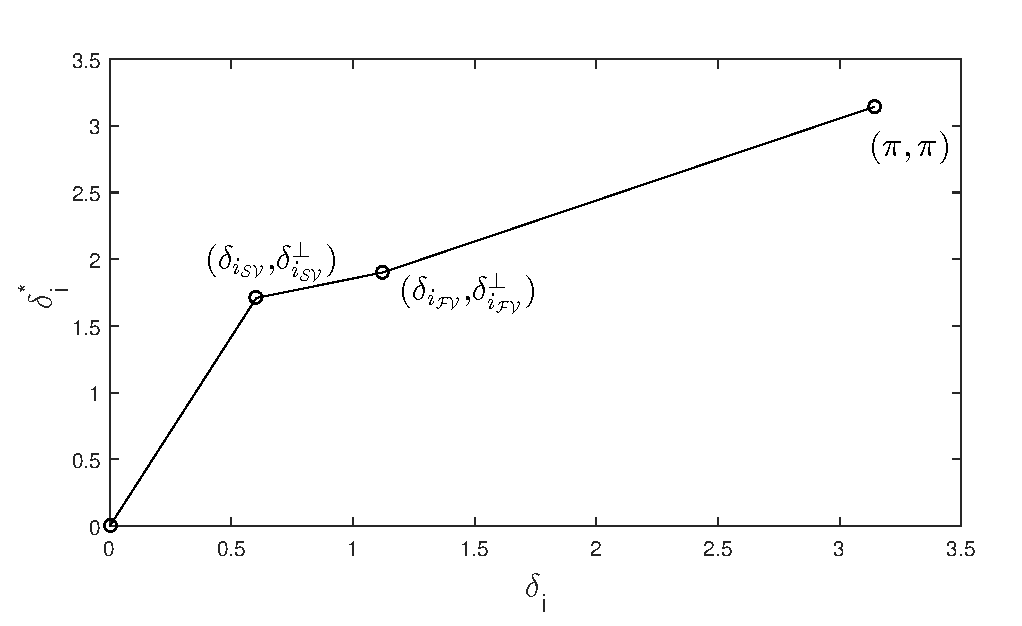
\includegraphics[scale=0.7]{Fig/simple_spline1.pdf}
\caption{The simple mapping function.}
%figure;plot([0,close,1.12,pi], [0,closed,1.9,pi],'-ko')
\label{fig:simple_spline}
\end{figure}

\section{Optimized Mapping Function}

The mapping function in Fig.\ref{fig:simple_spline} demonstrates monotonicity and continuity, which is a part of targeted characteristics as an ideal mapping function for $f_i$. However there exists some drawbacks in the simple mapping function. First of all, the function is not differentiable at two target points ($\delta_{i_{{\mathcal{SV}}}}$,$\delta^{\perp}_{i_{{\mathcal{SV}}}}$) and ($\delta_{i_{{\mathcal{FV}}}}$,$\delta^{\perp}_{i_{{\mathcal{FV}}}}$), which will lead to cluster deformation. Secondly, since the mapping function is applied on the angular dimensions, linearity of each spline in the function will lead to non-convex clusters in Cartesian coordinates after mapping. In order to avoid deformations and preserve within cluster geometry, it is required to assign a region for each cluster within which the function maps the data to a equal or even smaller range in Cartesian coordinates. In other words, the samples close to the centroids has to be close to the same corresponding centroids in the mapped space. In order to avoid deformations, an optimized mapping function is proposed in this section.

To compromise three constrains, a function which satisfies the following mathematical conditions is studies:

\begin{itemize}
\item mapping function derivatives around centroids 0 and $\delta_{i_{{\mathcal{SV}}}}$ and $\delta_{i_{{\mathcal{FV}}}}$ are small
\item mapping function derivatives between two centroids large
\item quasi differentiable at all points
\end{itemize}

Therefore, we proposed the basis function $p$, which satisfies the aforementioned conditions. The function $p$ is composed of two parts: $h(x)$ and $g(x)$. The boundaries that each function activates are decided by target points ($\delta_{i_{{\mathcal{SV}}}}$,$\delta^{\perp}_{i_{{\mathcal{SV}}}}$) and ($\delta_{i_{{\mathcal{FV}}}}$,$\delta^{\perp}_{i_{{\mathcal{FV}}}}$) along with the mid-points between the target points. The lower boundary mid points are noted as ($\gamma$,$\gamma^{\perp}$). The upper boundary mid points are noted as ($\epsilon$,$\epsilon^{\perp}$). To ensure the continuity of the mapping function $f$, the boundaries and target points satisfy:

\begin{align}
\begin{aligned}
(\epsilon_{i_{{\mathcal{SV}}}},\epsilon^{\perp}_{i_{{\mathcal{SV}}}}) &=
(\gamma_{i_{{\mathcal{FV}}}},\gamma^{\perp}_{i_{{\mathcal{FV}}}}) &=
(\frac{\delta_{i_{{\mathcal{SV}}}} + \delta_{i_{{\mathcal{FV}}}}}{2}, \frac{\delta^{\perp}_{i_{{\mathcal{SV}}}} + \delta^{\perp}_{i_{{\mathcal{FV}}}}}{2})
\end{aligned}
\end{align}

Therefore, the two piecewise functions $h(x)$ and $g(x)$ are defined as follows:

\begin{align}
K_h &= \frac{\epsilon^{\perp}-\delta^{\perp}}{e^{\alpha(\epsilon-\delta,0)^{+}}-1}\\ \nonumber
h(x) &= K_h[e^{\alpha(x-\delta,0)^{+}}-1] + \delta^{\perp}
\end{align}
\begin{align}
K_g &= \frac{\gamma^{\perp}-\delta^{\perp}}{e^{\alpha(-\gamma+\delta,0)^{+}}-1}\\ \nonumber
g(x) &= K_g[e^{\alpha(\delta-x,0)^{+}}-1] + \delta^{\perp}
\end{align}

To demonstrate this process, we first apply $p$ on two target points ($\delta_{i_{{\mathcal{SV}}}}$,$\delta^{\perp}_{i_{{\mathcal{SV}}}}$) and ($\delta_{i_{{\mathcal{FV}}}}$,$\delta^{\perp}_{i_{{\mathcal{FV}}}}$). This will result in a smooth curve as shown in Fig.\ref{fig:optimized_p}

\begin{figure}[t]
\centering
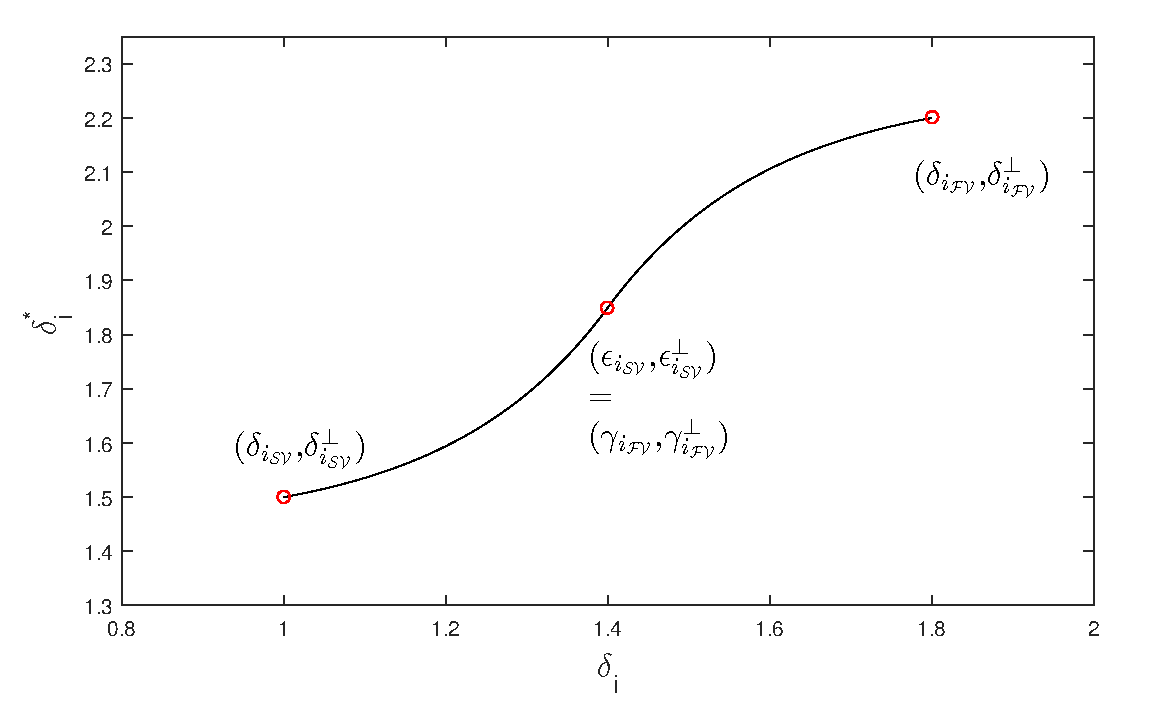
\includegraphics[scale=.7]{Fig/optimized_single_f.pdf}
\caption{Optimized Piecewise Interpolate Function $p$.}
\label{fig:optimized_p}
\end{figure}

Therefore, if we apply the piecewise interpolate function $p$ at all four target points: ($\delta_{i_{{\mathcal{SV}}}}$,$\delta^{\perp}_{i_{{\mathcal{SV}}}}$), ($\delta_{i_{{\mathcal{FV}}}}$,$\delta^{\perp}_{i_{{\mathcal{FV}}}}$) and two boundary points of angular dimension, the final result is shown in Fig.\ref{fig:optimized_map}

\begin{figure}[t]
\centering
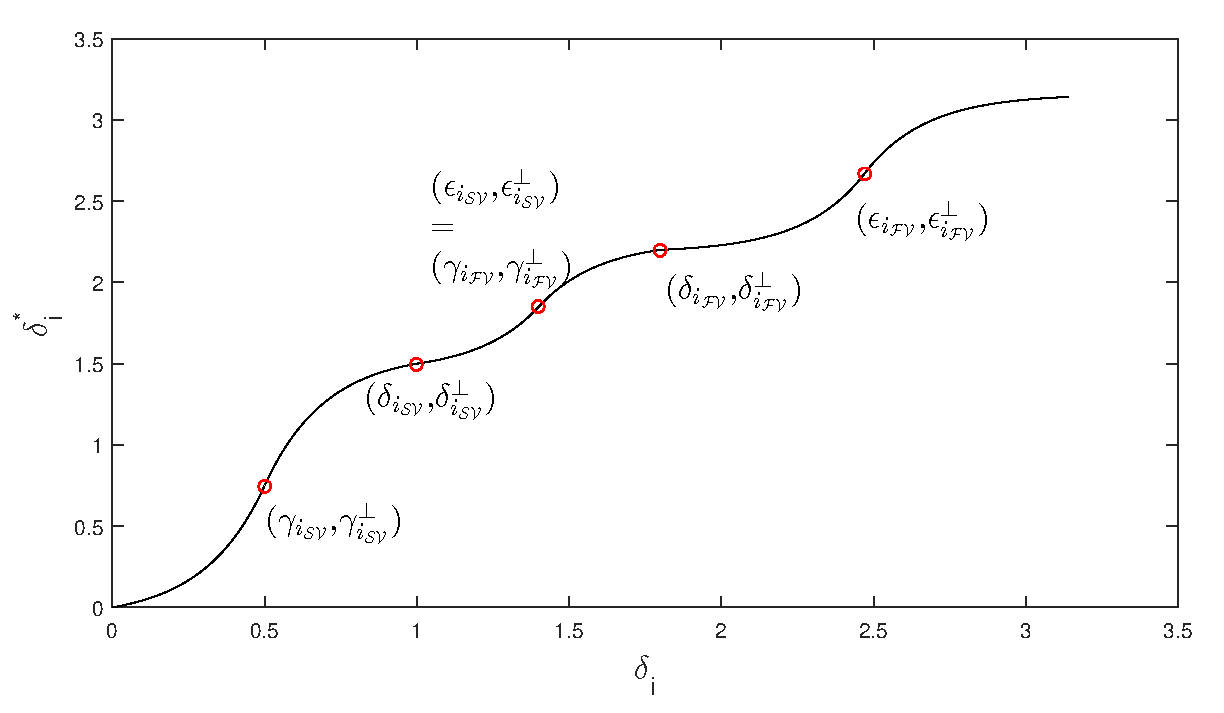
\includegraphics[scale=.7]{Fig/optimized_mapping_f.pdf}
\caption{Optimized Mapping Function $f$.}
\label{fig:optimized_map}
\end{figure}

In the training process, abnormal data from DS1 and personalized normal cluster are used to determine the mapping function. In the predicting process, the hyper-spherical coordinate of a new ECG sample is calculated and the mapping function is applied on its hyper-spherical coordinate. After this step, we calculate the Cartesian coordinate of the transformed data. This final result in Cartesian coordinate is then fed into Eq. \ref{eq:personal_discrim} to generate the corresponding type of yellow alarm.

\section{Experimental Results}\label{sec:result_spatial}

In this section, the performance of proposed method is evaluated according to two aspects. We will first analyze the classification performance of the system and demonstrate the comparison with other representative ECG classifiers. Furthermore, the classification results are partitioned into two sets:  red alarms generated by global classifier and final results by combining yellow and red alarms. In this way, the impacts of personalized classifier on final results can be revealed. Finally, the prediction performance which is representative in the proposed system is evaluated.

\subsection{Classification Performance}

The experimental results are evaluated with the classification performance of 4 AAMI ECG classes using the test subset of MITBIH Arrhythmia DS2. Originally DS2 contains 15357 samples after feature extraction. While training Personal Classifier, the first 20\% of total normal samples serve as initialization samples for personalized dynamic normal cluster. Therefore, all samples before the last initialization normal sample should be excluded from test set for each records. Consequently, the actual test set contains 12414 samples in total consisting of 10105 type-N, 1702 type-V, 508 type-S and 99 type-F samples.

To present the result, we select weighted k-Nearest Neighbors where $k=10$ as global classifier because it's comparatively simple and representative among low complexity models. The parameter $\alpha$ in the deviation detection module is set to 1 for test purpose. 

Table \ref{table:classification_cumu} summarized the cumulated confusion matrix for all records in the test set. In order to compare the result of global classifier and combined result, the sample numbers are presented in the following format: $combined(globaled)$. In order to measure classification performance, we adopted three metrics proposed in \cite{Hu_et_al,deChazal2006,ince2009generic}: accuracy($Ac$), sensitivity($Se$), specificity($Sp$). All three metrics are calculated based on true positive $TP$, false positive $FP$, false negative $FN$ and true negative $TN$ in a binary confusion matrix. Therefore all four metrics are calculated for each class by converting the 4x4 matrix to a 2x2 matrix.

\begin{table}[t]
	\centering
	\caption{Cumulated Confusion Matrix for All Records in DS2}
	\vspace{-0.05in}
	\begin{tabular}{|l|l|c|c|c|c|}
		\hline 
		&  \multicolumn{4}{c}{Ground Truth} &\\ 
        \hline
		\multirow{5}{*}{Result} &  & N & V & S & F  \\\cline{2-6}
		& N & 9255(10076)& 21(38) & 72(90) & 1(5) \\\cline{2-6} 
		&V & 657(22) & 1678(1663) & 8(2) & 9(7)  \\\cline{2-6}
		&S & 71(6) & 3(1) & 417(416) & 0(0)  \\\cline{2-6}
        &F& 122(1) & 0(0) & 11(0) & 89(87)  \\\hline
	\end{tabular}
	\label{table:classification_cumu} 
	\vspace{-0.15in}
\end{table}

While cumulated classification results are demonstrated in Table \ref{table:classification_cumu}, the robustness of the proposed method should be evaluated based on the performance variation over 22 test records in DS2. Hence medians and IQRs(interquartile range) for each metric and each class are included in Table \ref{table:variation} to represent the robustness of proposed methods. The lower variation between performances measured on different tapes, the more robust the system is. In Table \ref{table:variation}, we observe that among all abnormal classes, the proposed method demonstrates stable performance on class V but less stable on class S and F.

\begin{table}[b]
\centering
\caption{Classification Performance and Within-Set Variation of Proposed System}
\label{table:variation}
\resizebox{\textwidth}{!}{
\begin{tabular}{|c|c|c|c|c|c|c|c|c|c|c|c|c|}
\hline
\multirow{2}{*}{statistics} & \multicolumn{3}{c|}{N}                  & \multicolumn{3}{c|}{V}                  & \multicolumn{3}{c|}{S}                  & \multicolumn{3}{c|}{F}                  \\ \cline{2-13} 
                            & \textit{Ac} & \textit{Se} & \textit{Sp} & \textit{Ac} & \textit{Se} & \textit{Sp} & \textit{Ac} & \textit{Se} & \textit{Sp} & \textit{Ac} & \textit{Se} & \textit{Sp} \\ \hline
cumulated                   & 92.4        & 91.59       & 95.93       & 94.38       & 98.59       & 93.71       & 98.67       & 82.09       & 99.38       & 98.85       & 89.9        & 98.92       \\ \hline
median                      & 94.45       & 92.21       & 95.42       & 96.17       & 99.55       & 95.71       & 99.38       & 80.65       & 99.84       & 99.11       & 90.91       & 99.11       \\ \hline
IQR                         & 6.33        & 10.08       & 11.91       & 5.17        & 1.64        & 8.62        & 1.76        & 19.35       & 0.61        & 1.58        & 23.33       & 1.49        \\ \hline
\end{tabular}}
\end{table}

As MITDB is widely used to verify ECG classifier performance, we compared the proposed system with five significant methods proposed in literature. According to AAMI standards, ECG classifier performance should be evaluated over the binary classification performance of \textit{Ventricular (V)} versus \textit{non-V}types and \textit{Supraventricular (S)} versus \textit{non-S} types. For methods proposed in literature, same evaluation metrics are deployed on records from MITDB. To standardize the metrics, we select 11 common ECG records from all 5 methods and compared the median of each classification metrics over these 11 records. The comparison results are demonstrated in Table \ref{table:classification_comp}. Generally speaking, the proposed method shows higher sensitivity for both V type and S type. Especially for S type, the proposed method has advantage on all three metrics over other five methods in the literature.


\begin{table}[tbp]
\centering
\caption{V and S classification performance compared with five algorithms in literature using 11 common records in MITDB}
\label{table:classification_comp}
\begin{tabular}{|c|c|c|c|c|c|c|}
\hline
\multirow{2}{*}{Methods} & \multicolumn{3}{c|}{VEB} & \multicolumn{3}{c|}{SVEB} \\ \cline{2-7} 
                         & Ac     & Se     & Sp     & Ac      & Se     & Sp     \\ \hline
Proposed                 & 96.6   & 98.2   & 92.4   & 98.63   & 88.89  & 99.41  \\ \hline
Hu \textit{et al.}\cite{Hu_et_al}     & 94.8   & 78.9   & 96.8   & N/A     & N/A    & N/A    \\ \hline
de Chazal \textit{et al.}\cite{autofs}  & 96.4   & 77.5   & N/A    & N/A     & N/A    & N/A    \\ \hline
Jiang and Kong \cite{bbnn}    & 98.8   & 78.9   & 96.8   & 97.5    & 74.9   & 98.8   \\ \hline
Ince \textit{et al.} \cite{ince2009generic}    & 97.9   & 90.3   & 98.8   & 96.1    & 81.8   & 98.5   \\ \hline
Kiranyaz \textit{et al.}\cite{Kiranyaz}         & 98.9   & 95.9   & 99.4   & 96.4    & 68.8   & 99.5   \\ \hline
\end{tabular}
\end{table}

\subsection{Prediction Performance}

As an important characteristic of the proposed methods, yellow alarms triggered by personalized classifier after feature space reshaping indicate a higher probability of observing subsequent abnormalities. In order to verify this functionality, all beats following a yellow alarm is investigated for each yellow alarm. Abnormality type which occurs the earliest within the window is recorded. Similar to confusion matrix for classification evaluation, the performance of prediction can be summarized by a confusion matrix with the 3 abnormal types. Probabilities of observing a certain type of abnormal beats after a yellow alarm is calculated using the prediction confusion matrix and compared to the prior probability of observing the same type of abnormality. This process is formulated in the following two equations:

\begin{align}
\nonumber 
&P(\hat{y}_{k+i}=X_r|\hat{y}_{k}=X_y)=\frac{\text{\# of $y_{k+i}=X$ after $\hat{y}_k=X_y$}}{\text{\# of true alarms after $\hat{y}_k=X_y$}} \\
&P(\hat{y}_{k+i}=X_r)=\frac{\text{\# of true alarm of type $X$ ($y_{k}=X$)}}{\text{\# of all true alarms}} 
\end{align}

The power of predicting each type of abnormalities is evaluated by comparing $P(\hat{y}_{k+i}=X_r|\hat{y}_{k}=X_y)$ and $P(\hat{y}_{k+i}=X_r)$. A shown in Table \ref{table:pred}, the probability of observing a certain type of abnormalities after a yellow alarm is higher than its prior for each type of abnormalities. For example, without knowing the type of a yellow alarm, the probability of observing a type $V$ sample is 71.54\% while the probability of observing a type $V$ sample given a type $V$ yellow alarm was triggered is 77.45\%. The improvement are consistent among all three types of abnormalities but the system has stronger predicting capacity for type $S$. 

\begin{table}[t]
\centering
\caption{predictive probability versus prior probability without windowing}
\label{table:pred}
\begin{tabular}{|c|l|l|l|l||l|l|l|}
\hline
\multicolumn{2}{|l|}{\multirow{2}{*}{}} & \multicolumn{3}{l|}{\# of predicted ground truth} & \multicolumn{3}{l|}{\% of predicted ground truth} \\ \cline{3-8} 
\multicolumn{2}{|l|}{}                  & V               & S               & F             & V               & S               & F             \\ \hline
\multirow{3}{*}{yellow alarm}    & V    & 467             & 122              & 14            & \textbf{77.45}  & 20.23           & 2.32          \\ \cline{2-8} 
                                 & S    & 36              & 15              & 0             & 70.59           & \textbf{28.41}  & 0             \\ \cline{2-8} 
                                 & F    & 40              & 60              & 5             & 38.10           & 57.14           & \textbf{4.76} \\ \hline
\multicolumn{2}{|c|}{total}             & 543             & 197             & 19            & \textbf{71.54}  & \textbf{25.96}  & \textbf{2.50} \\ \hline
\end{tabular}
\end{table}

In order to study the time window in which real abnormality occurs after yellow alarms, we also studied a window of 10 consecutive samples following a yellow alarm. Similarly, prior and posterior probabilities are compared to evaluate the performance as shown in Table.\ref{table:pred10}. 


\begin{table}[t]
\centering
\caption{predictive probability versus prior probability within 10 beats' window}
\label{table:pred10}
\begin{tabular}{|c|l|l|l|l||l|l|l|}
\hline
\multicolumn{2}{|l|}{\multirow{2}{*}{}} & \multicolumn{3}{l|}{\# of predicted ground truth} & \multicolumn{3}{l|}{\% of predicted ground truth} \\ \cline{3-8} 
\multicolumn{2}{|l|}{}                  & V               & S               & F             & V               & S               & F             \\ \hline
\multirow{3}{*}{yellow alarm}    & V    & 290             & 85              & 12            & \textbf{74.94}  & 21.96           & 3.10          \\ \cline{2-8} 
                                 & S    & 22              & 13              & 0             & 62.86           & \textbf{37.14}  & 0             \\ \cline{2-8} 
                                 & F    & 29              & 37              & 6             & 40.28           & 51.39           & \textbf{8.33} \\ \hline
\multicolumn{2}{|c|}{total}             & 341             & 135             & 18            & \textbf{69.03}  & \textbf{27.32}  & \textbf{3.64} \\ \hline
\end{tabular}
\end{table}

Compared with the result without windowing, the predicting performance within 10 beats window shows that the proposed algorithm can better predict the occurrence of abnormalities in a certain time window. Especially for type S, the probability of observing a type S sample within 10 beats after a yellow alarm is 27.32\% while given that the yellow alarm is type S, the posterior probability is raise to 37.14\%. With almost 10\% increase, it's proved that the yellow alarm types are informative. The results shows that same improvements are made within the 10-sample window as well. In general, the predicting performance are promising, indicating the efficiency of personalized classifier and deviation analysis.